\documentclass[a4paper, man, floatsintext]{apa6}
\usepackage{lmodern}
\usepackage{amssymb,amsmath}
\usepackage{ifxetex,ifluatex}
\usepackage{fixltx2e} % provides \textsubscript
\ifnum 0\ifxetex 1\fi\ifluatex 1\fi=0 % if pdftex
  \usepackage[T1]{fontenc}
  \usepackage[utf8]{inputenc}
\else % if luatex or xelatex
  \ifxetex
    \usepackage{mathspec}
  \else
    \usepackage{fontspec}
  \fi
  \defaultfontfeatures{Ligatures=TeX,Scale=MatchLowercase}
\fi
% use upquote if available, for straight quotes in verbatim environments
\IfFileExists{upquote.sty}{\usepackage{upquote}}{}
% use microtype if available
\IfFileExists{microtype.sty}{%
\usepackage{microtype}
\UseMicrotypeSet[protrusion]{basicmath} % disable protrusion for tt fonts
}{}
\usepackage{hyperref}
\hypersetup{unicode=true,
            pdfauthor={Jana B. Jarecki},
            pdfborder={0 0 0},
            breaklinks=true}
\urlstyle{same}  % don't use monospace font for urls
\usepackage{graphicx,grffile}
\makeatletter
\def\maxwidth{\ifdim\Gin@nat@width>\linewidth\linewidth\else\Gin@nat@width\fi}
\def\maxheight{\ifdim\Gin@nat@height>\textheight\textheight\else\Gin@nat@height\fi}
\makeatother
% Scale images if necessary, so that they will not overflow the page
% margins by default, and it is still possible to overwrite the defaults
% using explicit options in \includegraphics[width, height, ...]{}
\setkeys{Gin}{width=\maxwidth,height=\maxheight,keepaspectratio}
\IfFileExists{parskip.sty}{%
\usepackage{parskip}
}{% else
\setlength{\parindent}{0pt}
\setlength{\parskip}{6pt plus 2pt minus 1pt}
}
\setlength{\emergencystretch}{3em}  % prevent overfull lines
\providecommand{\tightlist}{%
  \setlength{\itemsep}{0pt}\setlength{\parskip}{0pt}}
\setcounter{secnumdepth}{0}
% Redefines (sub)paragraphs to behave more like sections
\ifx\paragraph\undefined\else
\let\oldparagraph\paragraph
\renewcommand{\paragraph}[1]{\oldparagraph{#1}\mbox{}}
\fi
\ifx\subparagraph\undefined\else
\let\oldsubparagraph\subparagraph
\renewcommand{\subparagraph}[1]{\oldsubparagraph{#1}\mbox{}}
\fi

%%% Use protect on footnotes to avoid problems with footnotes in titles
\let\rmarkdownfootnote\footnote%
\def\footnote{\protect\rmarkdownfootnote}

%%% Change title format to be more compact
\usepackage{titling}

% Create subtitle command for use in maketitle
\providecommand{\subtitle}[1]{
  \posttitle{
    \begin{center}\large#1\end{center}
    }
}

\setlength{\droptitle}{-2em}

  \title{}
    \pretitle{\vspace{\droptitle}}
  \posttitle{}
    \author{Jana B. Jarecki}
    \preauthor{\centering\large\emph}
  \postauthor{\par}
      \predate{\centering\large\emph}
  \postdate{\par}
    \date{20 November, 2019}

\usepackage{natbib} \usepackage{threeparttable} \usepackage{booktabs}
\shorttitle{test} \usepackage{setspace}
\AtBeginEnvironment{tabular}{\singlespacing} \usepackage{times}
\usepackage{changes} \definechangesauthor[name={JJ}, color=orange]{jj}
\usepackage{upgreek} \AtBeginDocument{\let\maketitle\relax}

\begin{document}

\subsubsection{Qualitative predictions of the cognitive models}
\added[id=jj]{The next analyses focus on qualitative predictions from the cognitive strategies. For these analyses we pooled the observed data from both studies ($N=80$) and used the participants' best-fitting models from the cognitive modeling.}

\textit{Effects on evaluations.} In our task, the relative frequency
model predicts that sample size will not affect evaluations (the
relative frequencies were identical across sample sizes). In contrast,
the Bayesian value updating model predicts that given different prior
beliefs the frequency of experienced outcomes will change peoples'
beliefs in different directions, and that this change is stronger with
larger sample size. According to the Bayesian value updating model,
participants with a zero-outcome prior who sample p-bets should increase
their evaluations with higher sample size, but participants with a gain
prior who sample \$-bets should decrease their evaluations with higher
sample size. To test these hypotheses, participants were classified as
relative-frequency learners, Bayesians with gain priors
\(\theta_G > 1\), and Bayesians with zero-outcome priors
\(\theta_G \leq 1\), based on the individually best-fitting cognitive
model. Figure \ref{fig:fig6}a shows that, as predicted, among the
Bayesian participants, those with zero-outcome priors increased their
evaluations of p-bets, those with gain priors decreased their
evaluations of \$-bets, and RF-type participants remained relatively
stable across sample sizes. Statistical analyses by means of a Bayesian
generalized linear
model\footnote{regressing the (normalized, within-person z-standardized) evaluations on the predictors sample size, gamble type, and learner class (BVU-gain-prior, BVU-loss-prior, RF) with a by-participant random intercept; categorical predictors were effects-coded to facilitate interpretation of interactions \citep[for details, see][]{SingmannForthcoming}}
favored a regression with the best-fitting cognitive model class as
predictor over a regression excluding the cognitive model class,
\(BF\textsubscript{01}=26\).

\begin{figure}[htb]

{\centering 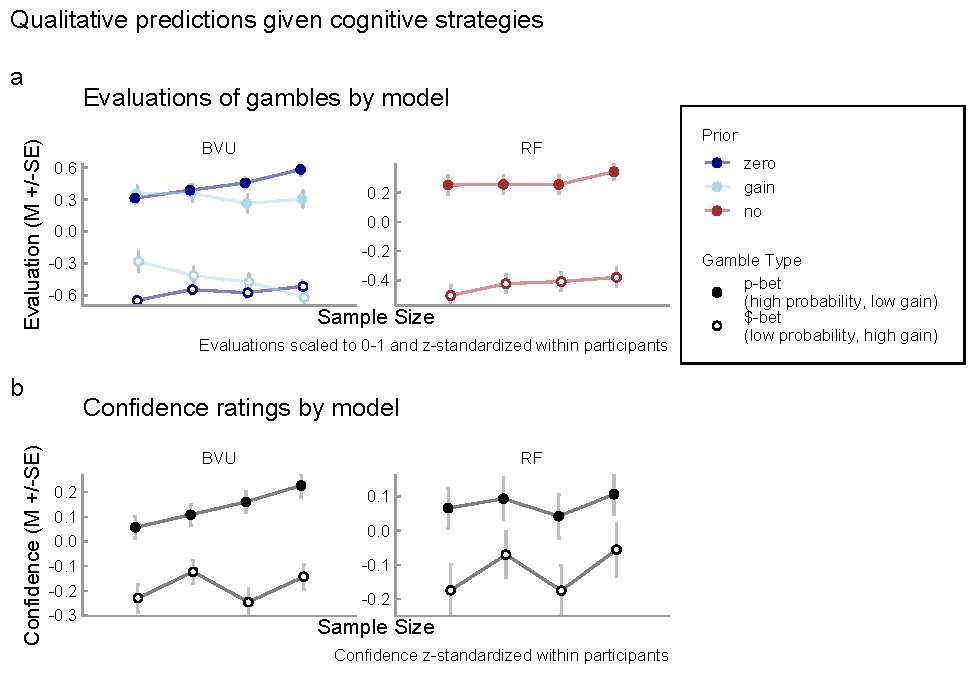
\includegraphics[width=.9\linewidth]{../figures/fig6-1} 

}

\caption{Mean evaluations by gamble type and best-fitting cognitive model and prior beliefs of the BVU model. \textit{BVU}$=$Bayesian value updating model, \textit{RF}$=$ Relative frequency model. Error bars indicate standard errors. Sample size categories see Table \ref{tab:Lotteries}. \textit{n} denotes the number of participants (of 80) that fall into the best-fitting model class. Evaluations are scaled to 0-1 and z-standardized at the individual level.}\label{fig:fig6}
\end{figure}

\textit{Effects on confidence.}
\added[id=jj]{Regarding uncertainty about beliefs, the Bayesian model predicts that more evidence decreases the uncertainty about beliefs. Thus confidence should increase with sample size for Bayesian learners. The relative frequency model makes no predictions about confidence. To test this, we classified participants into Bayesian and relative-frequency learners based on the best-fitting model. Contrary to the predictions, the Bayesian participants' confidence did not consistently increase with sample size (see Figure \ref{fig:fig6}b), and a linear model of confidence  predicted by sample size category and gambletype ($M_0$) fitted the data better than a model with the model-based classification as predictor ($BF_{01}> 1000$).}


\end{document}
